\documentclass[twoside,twocolumn]{article}
\usepackage{amsmath}
\usepackage{blindtext} % Package to generate dummy text throughout this template 
\usepackage{graphicx}
\usepackage{natbib}

\usepackage[sc]{mathpazo} % Use the Palatino font
\usepackage[T1]{fontenc} % Use 8-bit encoding that has 256 glyphs
\linespread{1.05} % Line spacing - Palatino needs more space between lines
\usepackage{microtype} % Slightly tweak font spacing for aesthetics

\usepackage[english]{babel} % Language hyphenation and typographical rules

\usepackage[hmarginratio=1:1,top=32mm,columnsep=20pt]{geometry} % Document margins
\usepackage[hang, small,labelfont=bf,up,textfont=it,up]{caption} % Custom captions under/above floats in tables or figures
\usepackage{booktabs} % Horizontal rules in tables

\usepackage{lettrine} % The lettrine is the first enlarged letter at the beginning of the text

\usepackage{enumitem} % Customized lists
\setlist[itemize]{noitemsep} % Make itemize lists more compact

\usepackage{abstract} % Allows abstract customization
\renewcommand{\abstractnamefont}{\normalfont\bfseries} % Set the "Abstract" text to bold
\renewcommand{\abstracttextfont}{\normalfont\small\itshape} % Set the abstract itself to small italic text

\usepackage{titlesec} % Allows customization of titles
\renewcommand\thesection{\Roman{section}} % Roman numerals for the sections
\renewcommand\thesubsection{\roman{subsection}}
\titleformat{\section}[block]{\large\scshape\centering}{\thesection.}{1em}{} % Change the look of the section titles
\titleformat{\subsection}[block]{\large}{\thesubsection.}{1em}{} % Change the look of the section titles

\usepackage{fancyhdr} % Headers and footers
\pagestyle{fancy} % All pages have headers and footers
\fancyhead{} % Blank out the default header
\fancyfoot{} % Blank out the default footer
\fancyhead[C]{FYS4150 $\bullet$ Project 3 $\bullet$ October 2016} % Custom header text
\fancyfoot[RO,LE]{\thepage} % Custom footer text

\usepackage{titling} % Customizing the title section

\usepackage{hyperref} % For hyperlinks in the PDF

%----------------------------------------------------------
%  COMMANDS
%---------------------------------------------------------

\newcommand{\nl}{
	
	\medskip
	\noindent
}
%--------------------------------------------

\newcommand{\SE}{Schroedinger equation }
\newcommand{\CI}{Coulomb interactions}
%----------------------------------------------------------------------------------------
%	TITLE SECTION
%----------------------------------------------------------------------------------------

\setlength{\droptitle}{-4\baselineskip} % Move the title up

\pretitle{\begin{center}\Huge\bfseries} % Article title formatting
	\posttitle{\end{center}} % Article title closing formatting
\title{FYS4150 - Project 3} % Article title
\author{%
	\textsc{Vegard R\o{}nning \& Heine H. Ness \& Sindre R. Bilden} \\[1ex] % Your name
	\normalsize University of Oslo \\ % Your institution
	\normalsize \href{mailto:vegard.ronning@fys.uio.no}{vegard.ronning@fys.uio.no}\ ; \href{mailto:h.h.ness@fys.uio.no}{h.h.ness@fys.uio.no}\ ; \href{mailto:s.r.bilden@fys.uio.no}{s.r.bilden@fys.uio.no}\\% Your email address
	\footnotesize \href{https://github.com/sindrerb/FYS4150-Collaboration/tree/master/Doc/Project3}{github.com/sindrerb/FYS4150-Collaboration/tree/master/Doc/Project3}
	%\and % Uncomment if 2 authors are required, duplicate these 4 lines if more
	%\textsc{Jane Smith}\thanks{Corresponding author} \\[1ex] % Second author's name
	%\normalsize University of Utah \\ % Second author's institution
	%\normalsize \href{mailto:jane@smith.com}{jane@smith.com} % Second author's email address
}
%----------------------------------------------------------------------------
\date{\today} % Leave empty to omit a date
\renewcommand{\maketitlehookd}{%
	\begin{abstract}
\vspace{-0.4cm} \blindtext
\vspace{-0.5cm}
	\end{abstract}
}

%----------------------------------------------------------------------------

\begin{document}
	
	% Print the title
	\maketitle
	
	%----------------------------------------------------------------------------
	%	ARTICLE CONTENTS
	%----------------------------------------------------------------------------
\vspace{-2cm}
	\section{Introduction}\vspace{-0.4cm}
	\lettrine[nindent=0em,lines=2]{Q}uantum \blindtext
	%----------------------------------------------------------------------------
	\section{Methods}
	\label{sec:methods}
	\blindtext
	%----------------------------------------------------------------------------
	\section{Implementation}
	\label{sec:implementation}
	\blindtext
All code and results are found in the GitHub repository \\
{\small \centering \href{https://github.com/sindrerb/FYS4150-Collaboration/tree/master/Doc/Project2}{github.com/sindrerb/FYS4150-Collaboration/}}
	\section{Results and discussion}
	\label{sec:results}
	\blindtext
	
	\begin{table}[h]
			\caption{Table showing the three lowest computed eigenvalues $\lambda$ with $N$ mesh points, compared to the exact $\lambda_0=3$,$\lambda_1=7$ and $\lambda_2=11$.}\label{tbl:convergence}
		\centering
		\begin{tabular}{|l|l|l|l|}\hline
			$N$ & $\lambda_0$ & $\lambda_1$ & $\lambda_2$\\ \hline
			10 & 2.68672 & 6.11302 & 11.0574\\
			50 & 2.98745 & 6.93692 & 10.8453\\
			100& 2.99687 & 6.98432 & 10.9617\\
			200& 2.99916 & 6.99610 & 10.9904\\
			300& 2.99961 & 6.99828 & 10.9958\\
			400& 2.99986 & 6.99903 & 10.9976\\
			500& 2.99993 & 6.99937 & 10.9986\\\hline
\end{tabular}
\end{table}
\begin{figure}[p]
%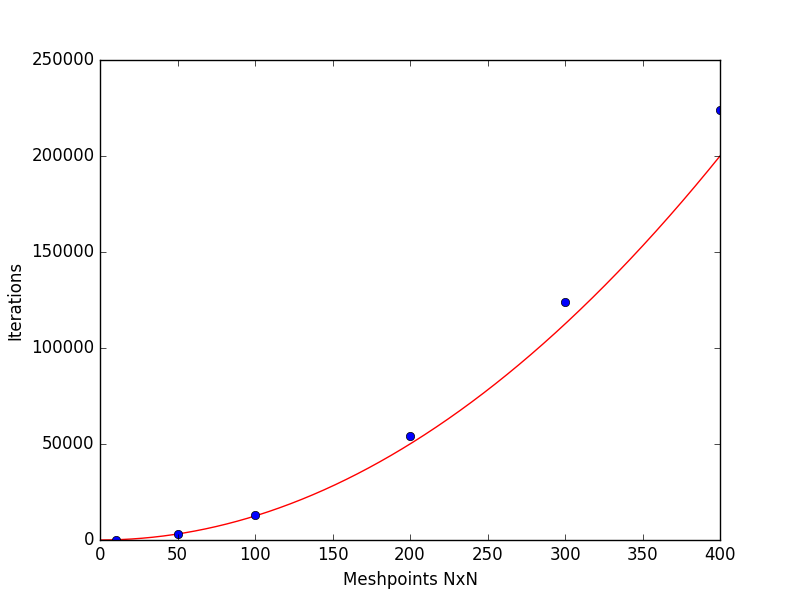
\includegraphics[width=0.5\textwidth]{figures/iterations.png} 
		\caption{Graph over the number of iterations for a given set of mesh points $N$. The solid red line is proportional to $N^2$ as a comparison.}\label{fig:iterations}
\end{figure}

\blindtext	%----------------------------------------------------------------------------
\section{Summary and Conclusion}
\label{sec:conclusion}
\blindtext	%----------------------------------------------------------------------------
	%\twocolumn[]
	
\end{document}